\documentclass[runningheads]{llncs}
%---- Sonderzeichen-------%
\usepackage[ngerman]{babel}
%---- Codierung----%
\usepackage[utf8]{inputenc}
%\usepackage[latin1]{inputenc}
\usepackage[T1]{fontenc}
\usepackage{graphicx}
\usepackage{url}
\usepackage{llncsdoc}
%----- Mathematischer Zeichenvorrat---%
\usepackage{amsmath}
\usepackage{amssymb}
\usepackage{enumerate}
\usepackage{nameref}
% fuer die aktuelle Zeit
\usepackage{listings}
\usepackage{textcomp}
\usepackage{color}
\usepackage{subfigure}
\usepackage{hyperref}
\usepackage[acronym,nomain]{glossaries}
\numberwithin{figure}{section}

\usepackage[citestyle=numeric,style=numeric,backend=biber]{biblatex}
\addbibresource{literature.bib}


\renewcommand{\labelitemi}{$\bullet$}
%\renewcommand{\thefigure}{\thesection-\arabic{figure}}

\setcounter{tocdepth}{3}
\setcounter{secnumdepth}{3}

% -------------------------------------------------------------------------------------------------
% -------------------------------------------------------------------------------------------------
\mainmatter
\title{5G Edge Cloud Architektur}
\titlerunning{5G Edge Cloud Architektur}
\author{Julian Beck}
\authorrunning{Julian Beck}
\institute{Betreuer: Prof. Dr. rer. nat. Oliver Waldhorst}
\date{01.05.2019}

\makeglossaries
\newacronym{mec}{MEC}{Multi-Access Edge Computing}
\newacronym{etsi}{ETSI}{European Telecommunications Standards Institute}
\newacronym{sdn}{SDN}{Software-Defined Networking}
\newacronym{nfv}{NFV}{Network Function Virtualization}
\newacronym{nfvi}{NFVi}{Network Function Virtualization Infrastructure}
\newacronym{amf}{AMF}{Core Access and Mobility Management Function}
\newacronym{ausf}{AUSF}{Authentication Server Function}
\newacronym{cp}{CP}{Control Pane}
\newacronym{up}{UP}{User Pane}
\newacronym{nef}{NEF}{Network Exposure Function}
\newacronym{nrf}{NRF}{Network Resource Funktion}

\newacronym{smf}{SMF}{Session Management Function}
\newacronym{udm}{UDM}{Unified Data Management}
\newacronym{upf}{UPF}{User Plane Function}
\newacronym{cups}{CUPS}{Control-/User Plane Separation}
\newacronym{pcf}{PCF}{Policy Control Function}
\newacronym{vnf}{VNF}{Virtualized Network Functions}
\newacronym{vm}{VM}{Virtuelle Maschine}
\newacronym{ran}{RAN}{Radio Access Networks}
\newacronym{3gpp}{3GPP}{3rd Generation Partnership Project}
\newacronym{oss}{OSS}{Operation Support System}
\newacronym{cfs}{CFS}{Customer Facing Service}
\newacronym{ue}{UE}{User Equipment}
\newacronym{dn}{DN}{Data Network}
\newacronym{sba}{SBA}{Service Based Architecture}
\newacronym{rnis}{RNIS}{Radio Network Information Service}
\newacronym{af}{AF}{Application Function}
\newacronym{meo}{MEO}{MEC- Orchestartor}
\newacronym{wan}{WAN}{Wide Area Network}
\newacronym{iot}{iot}{Internet of Things}










\begin{document}
\let\oldaddcontentsline\addcontentsline
\def\addcontentsline#1#2#3{}
\maketitle
\def\addcontentsline#1#2#3{\oldaddcontentsline{#1}{#2}{#3}}


% -------------------------------------------------------------------------------------------------

\begin{abstract}
  Die Edge Cloud wird in dem Zeitalter von 5G eine wichtige Rolle spielen. 
  Als ein Bestandteil der 5G-Netzwerkarchitektur bietet es nicht nur eine Vielzahl von Cloud-Ressourcen, sondern
  ermöglicht neue Plattformen für Drittanbieter und das Entwickeln von neuen Erfahrungen für den Nutzer.
  Multi-Access Edge Computing (MEC) bietet Speicher- und Rechenressourcen in der Nähe des Endgerätes, 
  eine besser Latenzzeit für mobile Endbenutzer und effizientere Nutzung des Mobile Backhaul-
  und Core Netzwerkes. Diese Seminararbeit erläutert, welche Technologien \acrfull{mec} ermöglicht und geht auf die Architekturen 
  hinter \Acrshort{mec} Computing ein.
\end{abstract}

% -------------------------------------------------------------------------------------------------
\tableofcontents 
\newpage
\printglossary[type=\acronymtype]
\newpage
% -------------------------------------------------------------------------------------------------

\section{Einleitung}
\label{sec:Einleitung}
In den letzten zehn Jahren haben Fortschritte im Cloud-Computing einen zentralisierten Ansatz für die Systemadministration und den 
Systembetrieb verfolgt. Edge Computing gilt dabei als eine Evolution der von Cloud Computing, in dem es das Hosten von Anwendung an den
Netzwerkrandes bringt, näher an den Benutzer und die Anwendungen die Daten generierten. 
Das Edge Computing ist eine der Schlüsseltechnologien der 5G-Mobilfunktechnik. 
Im Gegensatz zu den Mobilfunknetzwerken der dritten oder vierten Generation (3G oder 4G) ist die Unterstützung einer Edge Cloud 
von Beginn an in den 5G-Standards berücksichtigt und integriert wurden.
\\
\\
Die Abkürzungen MEC steht für Multi Access Edge Computing. Dabei handelt es sich um eine Computer Architektur,
die die Bereitstellung verteilter Services und Ressourcen an den Rand des Netzwerks verlegt. \acrshort{mec} wird vom
\acrfull{etsi} vorangetrieben und entwickelt. 
\\
\\
Im Zentrum der Technologie steht der MEC-Host. 
Er wird am Rande des Netzwerks (in der Nähe eines 5G Funkmast) installiert und stellt so Speicherplatz, 
Rechenleistung für Anwendungen zur Verfügung \ref{fig:mec-and-5g}. Dies hat folgende Vorteile: \cite{etsiETSIGSMEC}\cite{samikekkiwalterfeatherstoneyonggangfangpekkakuurealicelianuragranjanETSIMultiaccessEdge}
\begin{itemize}
  \item Reduzierter Datenverkehr im Kernnetzwerk
  \item Geringe Latenz und Datenverarbeitungszeit wegen dank der kurzen Distanz
  \item Hohe Verfügbarkeit
  \item Unterstützung für Echtzeitanwendungen.
\end{itemize}
Das Erfassen und Verarbeiten von Daten in der Nähe des Endgerät verbessert so 
die Latenz und eine Echtzeitleistung für Anwendungen mit hoher Bandbreite.
\\
\\
MEC ist eine Schlüsseltechnologie für 5G. 
Indem es die Latenzzeit signifikant reduziert, ist es für 5G-Szenarien so erfolgskritisch. 
Deshalb wurde in das 5G-Gesamtkonzept von Anfang an die Unterstützung des MEC-Konzepts integriert. 
Nur dank MEC lassen sich die verschiedenen 5G Anwendungen in vollem Umfang verwirklichen.
\\
\\
Mit der Hilfe des \acrfull{mec} verwandelt sich das 5G Mobilfunknetz in eine vielseitige Plattform zur Erbringung 
einer Vielzahl von Services. So ermöglicht MEC die Realisierung einer Vielzahl von Anwendungen: \cite{talebMultiAccessEdgeComputing23}\cite{depellegriniCompetitiveCachingContents2017}\cite{etsiMultiaccessEdgeComputing}
\begin{itemize}
  \item Smart Cities
  \item Vehicle-to-Vehcile, Vehicle-to-Infrastructure
  \item Smart Factories
  \item Cloud Gaming 
  \item Edge Video Caching
\end{itemize}
\begin{figure}
  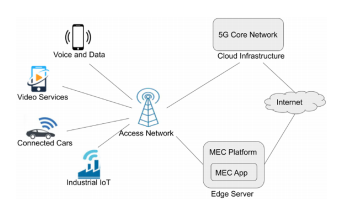
\includegraphics[width=\linewidth]{images/mec-and-5g.png}
  \caption{MEC und 5G}
  \label{fig:mec-and-5g}
\end{figure}
In dieser Arbeit wird in erster Linie auf die von \acrshort{etsi} veröffentlichte Architektur für ein MEC-System eingegangen.
\subsection{Aufbau der Seminararbeit}
Das zweite Kapitel dieser Seminararbeit \textbf{\nameref{sec:Benötigte Technologien} \ref{sec:Benötigte Technologien}} beschreibt
grundlegenden Technologien die für ein MEC System benötigt werden. Dazu zählt \acrfull{nfv}, \acrfull{sdn} aber auch die einzelnen  Komponenten in einem 5G System.
\\
\\
Das dritte Kapitel beschreibt die vom \acrlong{etsi} definierte Architektur eines MEC-Systems und die einzelnen Komponenten.
\\
\\
Im vierten Kapitel wird erläutert wie das MEC-System in 5G integriert wird und wie die einzelnen Komponenten mit einander kommunizieren.
\\
\\
Einer der wichtigsten Aspekte in einem Mobilen Netzwerk ist das Mobilitätsmanagement. Das vierte Kapitel beschreibt wie ein MEC-System mit der Mobilität von
Nutzern umgeht.
\\
\\
Das sechste Kapitel zeigt Szenarien in denen MEC eingesetzt werden kann. Es wird beispielsweise der eines MEC-Systems in einer Smart Factory und die daraus entstehnden
Vorteil erläutert.
\\
\\
Das letzte Kapitel zieht ein Fazit zum \acrlong{mec} und gibt ein Ausblick über die Zukunft der Technologie. 
Des Weiteren wird auf die aktuellen Probleme für das Einsetzen von \acrshort{mec} eingegangen.



\newpage
\section{Benötigte Technologien}
\label{sec:Benötigte Technologien}
Dieses Kapitel bietet eine kurze Einführung in die Kerntechnologien die die Anwendung eines 5G Netzwerkes erforderlich sind.
\subsection{Edge Computing}
\label{sub:Edge Computing}
Bei Cloud-Computing werden Rechenressourcen über ein Netzwerk zur Verfügung gestellt.
Beim Edge-Computing wird die Berechnung und Speicherung von Daten in die Nähe der Quelle gebracht,
an den sogenannten Rand oder \textit{Edge} des Netzwerks. Im Gegensatz zum Cloud-Computing werden die Daten
nicht in zentralen Rechenzentren verarbeitet, sondern an dezentralen Cloud Systemen am Rand des Netzwerks. 
Edge-Computing bietet dabei folgende Vorteile: \cite{inproceedings} \cite{labrieTopBenefitsEdge} 
\begin{itemize}
  \item \textbf{Geschwindigkeit und Latenz:} Abhängig von der Anwendungen spielt die Zeit der Datenverarbeitung eine
  entscheidende Rolle. Beispielsweise bei autonomen Fahrzeugen ist es wichtig, dass innerhalb von Millisekunden die Daten
  verarbeitet werden. Auch bei digitalen Fabriken ist es meist zu langsam die Daten zu einer zentralen Cloud und zurück
  zu senden. 
  Wenn die Datenverarbeitung auf den Rand des Netzwerks verlegt wird, wird die Latenz des Netzwerks verringert und schneller
  auf Anfragen geantwortet. 
  \item \textbf{Netzlast:} Da das die Daten nicht zu einer zentralen Cloud gesendet werden, sondern am Rand des Netzwerks 
  verarbeitet werden, verringert sich nicht nur die Latenz, sondern auch die Netzlast des gesamten Netzwerks. 
  Die Daten müssen nicht weitreichend weiter gesendet werden, stattdessen werden sie 
  dezentral in der Nähe der Anwendungen verarbeitet.
  \item \textbf{Security:} Wenn Daten in einer zentralen Cloud verarbeitet werden ist dies unter bestimmten Umständen anfälliger
  für ein Ausfall.
  So kann beispielsweise ein DDoS-Angriff den gesamten Betrieb eines Unternehmens blockieren, wenn alle Systeme mit einer zentralen
  Cloud arbeiten. Da bei Edge-Computing kein einziges zentrales Systeme existiert, verringert sich die Auswirkung eines solchen
  Angriffes für das ganze Unternehmen.  
  Edge Computing hilft Unternehmen auch dabei, die Probleme der lokalen Compliance- und Datenschutzbestimmungen zu überwinden,
  da die Daten auf lokalen Systemen verarbeitet werden.
  \item \textbf{Kosteneinsparungen:} Durch \acrfull{iot} Geräte oder durch eine Smart Factories werden
  eine Vielzahl an Daten generiert. Nicht alle Daten sind dabei kritisch für die Operation der Systeme. Edge Computing erlaubt
  das Kategorisieren der Daten. In dem ein Großteil der Verarbeitung am Rand des Netzwerks stattfindet wird Bandbreite gespart.
  Dies optimiert den Datenfluss von lokalen Anwendungen und minimiert so die Betriebskosten einer zentralen Cloud.
  \item \textbf{Zuverlässigkeit:} Wenn Edge-Geräte Daten lokal speichern und verarbeiten können, verbessert dies die Zuverlässigkeit.
  Ein Unternehmen ist nicht auf die Verbindung auf zur zentralen Cloud angewiesen und eine vorübergehende Unterbrechungen der 
  Verbindung hat keine Auswirkungen auf den Betrieb von Geräte, wenn diese die Verbindung zur Cloud verloren haben.
  \item \textbf{Skalierbarkeit:}
  Bei Cloud-Computing-Architekturen müssen Daten in den meisten Fällen zunächst an ein zentral gelegenes Rechenzentrum
  weitergeleitet werden. Das Erweitern oder das Ändern dedizierter Rechenzentren ist verursacht kosten. 
\end{itemize}
\subsection{5G Network}
\label{subsec:5G Network}
Das 5G-Netzwerk wurde entwickelt um auch von der Industrie genutzt zu werden.
Dies wird durch Techniken wie \acrlong{nfv} und \acrlong{sdn} ermöglicht. \cite{BARAKABITZE2020106984}
Klassischerweise wurden mobile Netzwekre in erster Linie für Endgeräte wie Smartphones und Laptop konzipiert. 
Dies ändert sich bei dem 5G Netzwerk. Durch eine Vielzahl von Anwendungen und unterschiedliche Anforderungen,
muss das Netzwerk so designt sein, dass es alle Forderungen der Industrie und des Endverbrauchers erfüllt. 
\\
\\
Um den neuen 5G-Anforderungen 10 Gbit/s Datenrate, 1 ms End-to-End-Latenz,  und 99:99\% 
Serviceverfügbarkeit gerecht zu werden setzt 5G auf Technologien wie \acrfull{cups}, \acrfull{nfv} und MEC.
\begin{figure}
  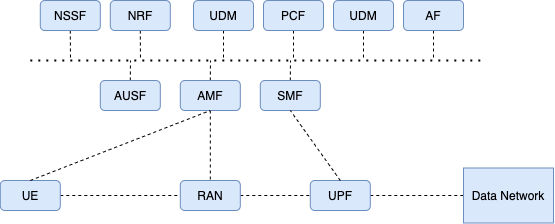
\includegraphics[width=\linewidth]{images/ServiceBased5g.png}
  \caption{Service Basierte Architektur}
  \label{fig:ServiceBased5g}
\end{figure}
\\
Die Darstellung \ref{fig:ServiceBased5g} zeigt die einzelnen Komponenten in Form einer Service basierten Architektur.  \cite{5GCoreNetwork2017}
Das 5G Netzwerk besteht aus sogenannten Netzwerkfunktionen, die meist softwarebasiert sind und so nach Bedarf angepasst/skaliert werden können.
Die 5G CP ist das Kernnetz, dass aus einer Reihe von Netzwerkfunktionen besteht, 
die für die Separierung, Priorisierung und Zugriffssteuerung erforderlich sind:
\begin{itemize}
  \item \textbf{\acrfull{ausf}} dient als Authentifizierungsserver
  \item \textbf{\acrfull{amf}} ist für die Integrität, Registrierungsmanagement, Verbindungsmanagement,
  Zugriffs und Securitymanagement zuständig
  \item \textbf{\acrfull{nef}} verbreiten von Funktionen und Events, 
  sichere Bereitstellung von Informationen aus externen Anwendungen für das \acrshort{3gpp}-Netzwerk. Diese Funktion ist vor allem für die Mobilität
  in der 5G Edge Cloud wichtig, was in Abschnitt \ref{sec:Mobilitätsmanagement} erläutert wird.
  \item \textbf{\acrfull{smf}} Sitzungsverwaltung, Zuweisung von IP Adressen an die Endgeräte. 
  \item \textbf{\acrfull{udm}} Generierung von Anmeldeinformationen für Authentifizierungen, 
  Verwalten der Benutzeridentifikation und Zugriffsautorisierung.
  \item \textbf{\acrfull{upf}} Datenrouting und Weiterleitung. Dateninspektionen. Die \acrshort{upf}s spielt eine zentrale Rolle für das Mobilitätsmanagement, was in 
  Kapitel \ref{sec:Mobilitätsmanagement} erleutert wird.
  \item \textbf{\acrfull{pcf}} Bereitstellung von Richtlinien für Funktionen, 
  Zugriff auf Abonnementinformationen
Bei der 5G Architektur sind die Netzwerkfunktionen der \acrfull{cp} von der \acrfull{up} getrennt, was als \acrfull{cups} bezeichnet wird.
Aufgaben der \acrshort{cp} ist das Verwalten der Benutzerverbindungen, Richtlinien sowie Authentifizierung während die \acrshort{up} für die 
Weiterleitung des Datenverkehrs zuständig ist.
Die Motivation hinter \acrshort{cups} ist die unabhängige Skalierung der \acrlong{up}, um den Netzwerkbetreibung eine flexible Dimensionierung
des Netzwerks zu ermöglichen. Wenn beispielsweise der Datenverkehr zunimmt, können \acrlong{upf} hinzugefügt werden, ohne die \acrlong{cp} zu beinträchtigen.
Teile der \acrshort{cp} Netzwerkfunktionen wie \acrshort{ausf}, \acrshort{pcf}, \acrshort{udm}, \acrshort{amf} und \acrshort{smf}. 
Zu der \acrshort{up} gehöret die \acrshort{upf}. \cite{5GCoreNetwork2017} \cite{5GCoreNetwork}
\end{itemize}


\subsection{Network Function Virtualization}
\label{subsec:Network Function Virtualization}
\acrfull{nfv} erlaubt es Netzwerkfunktionen, von der Hardware zu entkoppeln.
Dies ermöglicht das Verwenden von Gateways, Firewalls, DNS Services und Caching ohne proprietär Hardware.
\\
\\
Um ein neues Netwzerk zu erstellen, wird in der Regel eine Vielzahl von verschieden Hardware Komponenten benötigt. 
Diese benötigen Platz, Energie und müssen von qualifizierten Personal überwacht und gewartet werden. 
\acrlong{nfv} will dieses Problem lösen, indem mithilfe von Virtualisierungstechniken, Netzwerkfunktionen auf Standard
Server Hardware Komponenten betrieben werden. 
Folgende Vorteile werden durch NFV erziehlt: \cite{nfv_wp} \cite{etsiNetworkFunctionsVirtualisation}
\begin{itemize}
  \item \textbf{Skalierbarkeit und Flexibilität:} Die Virtualisierung erlaubt eine einfache Skalierung der Ressourcen.
  Bei einer großen Nachfrage eines Services kann dieser skaliert werden. Es können auch schnell weitere Instanzen einer Netzwerkfunktion gestartet werden.
  \item \textbf{Kosteneinsparungen:} Durch die Verwendung von Standard Komponenten werden die Kosten und der Energieverbrauch minimiert.
  \item \textbf{Anpassungsfähigkeit:} Die Virtualisierung erlaubt eine schnelle Anpassung an die Anforderungen eines Kunden. 
  Die Server können durch der Virtualiserung von mehreren Nutzern gleichzeitig verwendet werden und die Anforderungen des jeweiligen
  Kunden erfüllen. Dies wird auch als Network Slicing bezeichnet.
\end{itemize}


\subsubsection{NFV Architektur und Orchestration Framework:}
\acrshort{etsi} hat ein Standard für ein \acrshort{nfv} Framework veröffentlicht.
Dieser Standard definiert sogenannte \acrfull{vnf}, welche Netzwerkfunktionen in Software abbilden.
Die \acrshort{vnf} werden in der \acrfull{nfvi} veräfentlicht. Die \acrshort{nfvi} besteht aus gewöhnlichen
den Hardware Komponenten wie CPU und Speicher, aber auch einem Virtualisierungslayer. \\
Der \textit{NFV MANO} (NFV Management und Orchestrierung) Layer verwaltet die Infrastruktur und passt diese an die Anforderungen an.
Der \acrfull{vm} Lifecycle wird von \textit{NFV MANO} verwaltet, wenn eine \acrshort{vm} abstürzt wird sie durch diesen neugestartet.
\cite{etsiNetworkFunctionsVirtualisation}

\subsubsection{5G Edge Cloud und NFV}
Die \acrlong{nfv} spielt eine Schlüsselrolle für die Umsetzung einer 5G Edge Cloud.
\acrshort{nfv} erlaubt \textit{Network Slicing}, ein Aspekt der virtuellen Netzwerkarchitektur, 
mit dem mehrere virtuelle Netzwerke auf einer gemeinsam genutzten Infrastruktur bereitgestellt werden können. \cite{suzhiSpaceEdgeCloud2019}
\\
\\
\acrshort{nfv} ermöglicht die 5G-Virtualisierung, sodass physische Netzwerk in mehrere virtuelle Netzwerke unterteilt werden können. 
Dies erlaubt es unterschiedliche \acrfull{ran} verschiedene Arten von Diensten gleichzeitig anzubieten. 
Der Anwender merkt dabei kein Unterschied, da die \textit{Network Slicies} voneinander isoliert arbeiten. 
\acrshort{nfv} ist für die Skalierbarkeit, Flexibilität und Migration in einer 5G Edge Cloud wichtig. Wenn Anfragen an eine
Anwendung steigen, kann nicht nur die Ressourcen für diese Anwendung skaliert werden, sondern es kann auch durch das Hinzufügen weiterer
Software Instanzen in der \acrfull{nfvi}, die Netzwerkinfrastruktur mit skaliert werden. \cite{How5GNFV} \cite{etsiNetworkFunctionsVirtualisation}
\newpage
\subsection{Software-defined Networking}
\label{subsec:Software-defined Networking}
\begin{figure}[h]
  \centering
  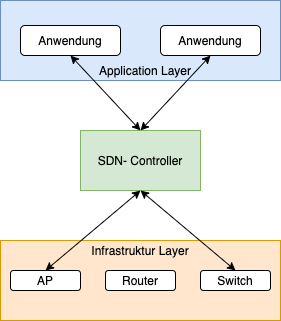
\includegraphics[width=6cm]{images/SDN.png}
  \caption{SDN Aufbau mit Northbound und Southbound API}
  \label{sdn1}
\end{figure}
Neben \acrshort{nfv}, ist auch \acrlong{sdn} für die Virtualisierung von Netzwerken wichtig.
Bei einem \acrshort{sdn} ist die Steuerung des Netzwerks von der Hardware getrennt. Es wird zwischen einem Controller, 
einer Southbound und einer Northbound API unterschieden. Die Northbound API, kommuniziert mit dem Application Layer,
die Southbound API mit dem Infrastruktur Layer,was in \ref{sdn1} zu sehen ist.
Die Southbound APIs führt die Anweisungen aus und gibt Informationen des Controllers an Netzwerkgeräte wie Switches,
Access Points und Router weiter. Der Controller ist das zentrale Element eines \acrshort{sdn} Netzwerkes, 
er ermöglicht ein zentrales Verwalten und Steuern des 
Netzwerkes. Die Northbound API gibt Informationen an den Controller weiter. Sie ist die Schnittstelle zwischen Anwendungen 
und dem \acrshort{sdn} Controller.\cite{SoftwareDefinedNetworkingSDN} \cite{arnold5GRadioAccess2017}
\\
\\
Das \acrlong{sdn} kann ein \acrshort{mec} unterstützen, indem es automatisch und flexibel Servicemanagement durchführt.
Da bei einem \acrshort{sdn} die \acrfull{up} und \acrfull{cp} durch die Southbound und Norhtbound API getrennt sind, 
führt \acrshort{sdn} eine zentrale Steuerung ein, 
mit der \acrshort{vnf} einfach gestartet und angeboten werden können. 
Die zugrunde liegende Netzwerkinfrastruktur wird so abstrahiert. Die Abstraktion von \acrshort{cp} und \acrshort{up} ermöglicht
im 5G eine bessere Implementation von \acrfull{cups}. Die Grafik \ref{fig:sdn2} zeigt die Controll-Netzwerkfunktionen von 5G in 
die über die Northbound API (NBI) mit dem SDN-Controller kommunizieren. Dieser steuert die \acrshort{up} des 5G Netzwerks über
die Southbound API (SBI).
Im Kontext von \acrshort{mec} kann der \acrshort{sdn}-Controller MEC bezogene \acrshort{vnf}, 
\acrshort{vm}s und Container als eine weitere Netzwerkkomponente behandeln, die dynamisch zugewiesen und neu lokalisiert werden können.
So kann der \acrshort{sdn}-Controller flexibel Services anpassen und dynamisch Dienste bereitstellen, 
indem er \acrshort{vnf}s und  \acrshort{mec} Dienste verbindet. Dies macht \acrshort{sdn} zu einem zentralen Element für die Virtualisierung
des MEC-Systems und für die Unterstützung der Mobilität.
\begin{figure}
  \centering
  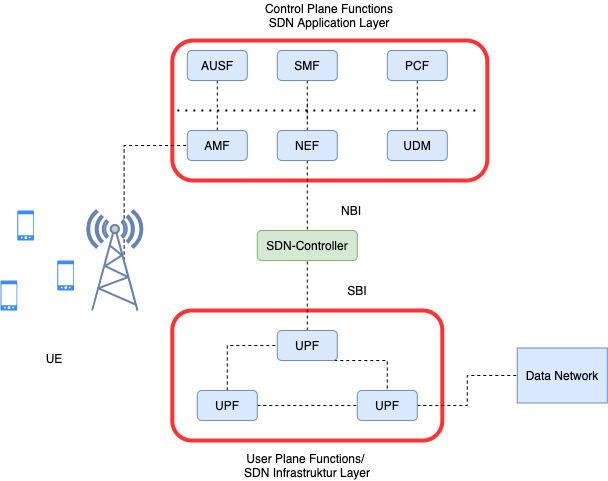
\includegraphics[width=11cm]{images/sdn2.png}
  \caption{SDN in einer 5G \acrshort{sba} Architektur}
  \label{fig:}
\end{figure}
Kommt es beispielsweise zu einer hohen Anfrage in einem 5G Netzwerk, wird das 5G-Netzwerk mittels \acrshort{nfv} Technologien skaliert.
\acrshort{sdn} hat dabei die Aufgabe des Load-balancings zwischen MEC-Anwendungen und Netzwerkfunktionen. Dies erlaubt das 
schnelle Erstellen und veröffentlichen neuer MEC-Komponenten wie MEC-Platform oder MEC-Anwendungen.
Die Kombination von \acrshort{sdn}s und \acrshort{nfv} erlaubt zusammen das Erstellen von \textit{Network Slices}. \cite{BARAKABITZE2020106984} 

\subsection{Virtuelle Maschinen und Container}
\label{subsec:Virtuelle Maschinen und Container}
Eine Cloud Plattform besteht typischerweise aus einer Anzahl von Maschinen, 
die durch einen Hypervisor zu einer zentralen Maschine zusammen gefasst werden.
Dieser kann isoliert virtuelle Maschinen erstellen und ausführen und dient als Abstraktionsebene, 
unabhängig von der Hardware auf denen die \acrshort{vm}s laufen.
\\
\\
Eine leichtgewichtigte Alternative zur Hypervisor-basierten Virtualisierung ist die Containergestützte Virtualisierung. 
Diese verwendet im Vergleich zu virtuellen Maschinen, eine andere Abstraktionsebene in Bezug auf Virtualisierung und Isolation. 
Container implementieren die Isolierung auf OS Ebene und vermeiden so die Virtualisierung von Hardware und Treibern. 
Insbesondere teilen sich Container denselben Kernel mit dem zugrunde liegenden Hostcomputer. 
Dies macht Container sehr leichtgewichtig und flexibel im 
Gegensatz zu VMs. Typischerweise führt ein Container genau ein Service aus, was eine schnelle Migration ermöglicht.
\\
\\
Im Blick auf \acrshort{mec} ermöglichen Container eine leichtgewichtige Virtualisierungslösung. So eigenen sich die Container
als eine portable Laufzeit Umgebung für MEC-Dienste. 
Einzelne Dienste können in Containern ausgeführt werden, sind so isoliert und können einfach 
verwaltet und gesteuert werden. Für die Umsetzung bietet sich die mittlerweile weitverbreitete Containerlösung Docker an. Hier stehen mit 
Kubernetes auch Orchestrierungs  und Clustering Tools zur Verfügung \cite{morabitoConsolidateIoTEdge2018}



\newpage
\section{MEC Framework und Referenz Architektur}
\label{subsec:MEC Framework - Referenz Architektur}
Folgendes Kapitel zeigt die vom \acrfull{etsi} beschriebene
Referenz Architektur zur Implementation eines \acrshort{mec} Systems. 
\\ 
\\
\acrshort{etsi} beschreibt dabei in ihrer Spezifikation \textit{Multi-access Edge Computing (MEC); 
Framework and Reference Architecture} \cite{etsiETSIGSMEC} ein Framework und eine 
Referenz Architektur. Die Grafik \ref{fig:MecFramework} zeigt das MEC-Framework. Dieses virtualisiert die essenziellen Komponenten eines 
MEC Systems.


\begin{figure}
  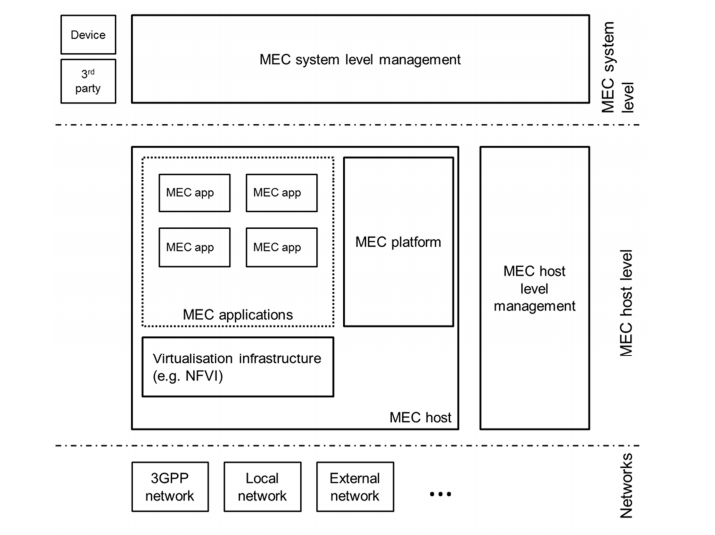
\includegraphics[width=\linewidth]{images/MecFramework.png}
  \caption{Multi-Access Edge Computing Framework \cite{etsiMultiaccessEdgeComputinga}}
  \label{fig:MecFramework}
\end{figure}

\subsection{Multi-access Edge Referenz Architektur}
Die Komponenten werden dabei auf Infrastruktur virtualisiert am Rande des Netzwerks ausgeführt. 
Dies ist möglich durch die in Kapitel \ref{sec:Benötigte Technologien} vorgestellten Technologien.
Die Grafik \ref{fig:mecarchitecture} zeigt die Komponenten der Referenz Architecture.
\begin{figure}
  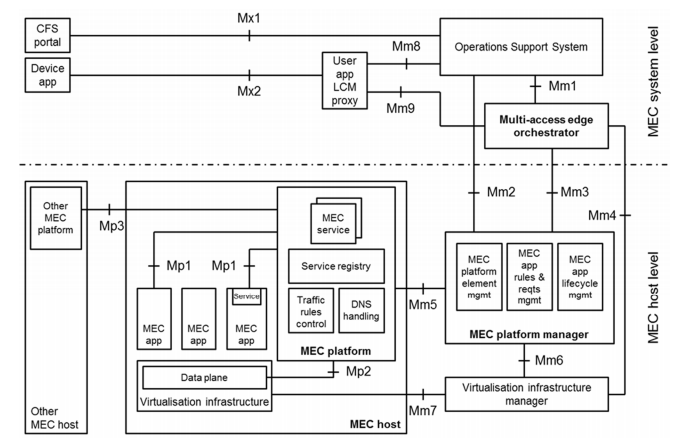
\includegraphics[width=\linewidth]{images/mecarchitecture.png}
  \caption{Multi-Access Edge System Reference Architecture \cite{etsiMultiaccessEdgeComputinga}}
  \label{fig:mecarchitecture}
\end{figure}
Die einzelnen Komponenten der MEC Framework und Referenz Architektur sind in folgende Ebenen unterteilt:
\subsubsection{Netzwerk Ebene}
Die unterste Ebene des Frameworks ist die Netzwerk Ebene. Sie ermöglicht die Verbindung zu dem lokalen und 
externen Netzwerk. Die \acrshort{3gpp} Komponente steht für \acrlong{3gpp}, was ein Überbegriff für mobilen
Telecommunications Standards wie LTE und 5G ist. 
\subsubsection{Distributed Host Level}
Wie der Name schon sagt, gibt es mehrere MEC-Hosts, die im Netzwerk Verteilt sind.
Der MEC Host enthält die MEC Platform und die Infrastruktur auf denen die Anwendungen, in der Edge Cloud, betreiben werden.
Die Infrastruktur stellt Rechen-, Speicher- und Netzwerkressourcen virtualisiert zu Verfügung. Als Virtualisierungslösung kann
die in Kapitel \ref{subsec:Network Function Virtualization} eingeführte \acrlong{nfvi}
eingesetzt werden. Der MEC-Host beinhaltet zwei weitere Komponenten:
\\
\\
\textbf{MEC-Platform:} Die MEC-Platform dient als eine art Registry für  
Anwendungen die auf der MEC Infrastruktur laufen. Die Plattform bietet eine Umgebung, in der MEC Anwendungen sich registieren,
und anderen Anwendungen Anfragen stellen können. Die MEC-Platform ist auch für DNS-Rekords zuständig. Sie nimmt Befehle
des MEC Platform Managers entgegen und passt die DNS Records und Proxies an. Des Weiteren verwaltet diese auch den Persistenten Speicher
\\
\\
\textbf{MEC-Anwendungen:} Multi-Access Edge Computing Anwendungen werden in einer Virtuellen Maschine oder als
Container auf der Infrastruktur des MEC-Hosts ausgeführt. Die Anwendungen registrieren sich bei der MEC Platform
Komponente, um darüber andere Anwendungen anzufragen und ihren Dienste zur Verfügung zu stellen. \cite{DevelopingSoftwareMultiAccess}
\\
\\
\textbf{MEC-Platform-Manager:} Der Platform-Manager verwaltet den Lifecycle der Anwendungen. Er startet, stoppt und startet diese neu.
Gleichzeitig informiert er den MEC-Orchestrator über wichtige Events der Anwendungen. 
Eine weitere Aufgabe ist das Verwalten, Managen und Autorisierung von DNS Configurationen.
Des Weiteren erhält der Platform Manager Fehlerberichte und Informationen über die Infrastruktur von dem Virtualisierungs Infrastruktur Manager.
\\
\\ 
\textbf{Virtualization-Infrastruktur-Manager:} Eine weitere Komponente im Host Level, ist der Virtualization-Infrastruktur-
Manager. Dieser ist für das Zuweisen, Verwalten und Freigeben von virtualisierten (Rechen-, Speicher- und Netzwerkressourcen)
Ressourcen der Virtualisierungsinfrastruktur zuständig. Der Manager ist dabei auch für das Konfigurieren der Infrastruktur für 
ein neues Software Image verantwortlich. Dazu gehört das Herunterladen und Speicheren der Images. Dabei kann der Manager auch 
Infrastructure-as-a-service Systeme wie Openstack unterstützen. Performance- und Fehlerdaten der Komponente werden von dem Manager gesammelt und weitergeleitet.
\\
\\
Kommt es zu einer Verschiebung einer Anwendung, wenn eine laufende Anwendung umgezogen wird,
interagiert der Virtualization Infrastruktur Manager mit dem MEC-Host zusammen um den Handoff an die neue Cloud durchzuführen.
Wie ein Handoff zwischen zwei MEC-Host abläuft wird in Kapitel \ref{sec:Mobilitätsmanagement} genauer erläutert.

\subsubsection{MEC System Level}
Das MEC System Level ist übergreifend über mehrere MEC-Hosts. 
\begin{figure}
  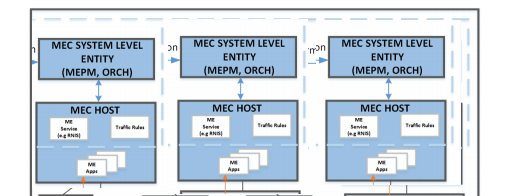
\includegraphics[width=\linewidth]{images/mec-System-Level.png}
  \caption{MEC-System Level übergreifend über mehrere MEC-Hosts}
  \label{fig:mec-System-Level}
\end{figure}
\textbf{MEC- Orchestrator:}
Der MEC-Orchestrator spielt eine zentrale Rolle, 
da er die Ressourcen und Funktionen des gesamten MEC-Systems im Blick hat. 
In vielerlei Hinsicht ähnelt dieser dem ETSI Network Functions Virtualization Orchestrator und hat ähnliche 
Aufgaben wie Orchestierung und Kontrolle der Instanziierung, Lösung von Ressourcenkonflikten.
Der MEC- Orchestartor ist verantwortlich für das Initialisieren, terminieren der Anwendungen, sowie das prüfen
der Integrität und Authentizität. Der Orchestrators stellt sicher, 
dass ein MEC- Host der die Anforderungen an die Anwendung wie Latenz und Verfügbaren Resourcen erfüllt, ausgewählt wird.
Ist dies nicht der Fall ist es auch Aufgabe des Orchestartor, ein besseren Host zu finden und die Anwendungen zu migrieren.
\\
\\
\textbf{Operations Support System:}
Das \acrfull{oss} ist die höchste Ebene, die eine Anwendung bei der Ausführung an einem Standort unterstützt. 
Das \acrshort{oss} empfängt Anforderungen zum Instanziieren und Beenden der mobilen Edge-Anwendungen von dem \acrfull{cfs} und von den Endgeräten.
Um diese zu erfüllen kommuniziert das Operation Support System mit dem MEC-Orchestartor.
\\
\\
\textbf{Customer Facing Service:}
Der \acrfull{cfs} dient als Schnittstelle für Drittanbieter und ähnelt Portalen wie bei Cloud-Plattformen. 
Dieser kommuniziert mit dem \acrshort{oss}.
\\
\\
\textbf{User App Lifecycle Management Proxy:} 
Der User App Lifecycle Management Proxy (User App LCM Proxy) ist eine Funktion, die Endgeräte anfordern können für Onboarding, Initalisierung und Terminierung der auf der
Edge-Cloud laufenden Services. Stellt eine Endgerät eine Anfrage, autorisiert der Proxy die Anfrage und leitet diese an das \acrshort{oss} und den MEC- Orchestrator weiter. 
Die Endgeräte können so mit dem MEC- System über den Proxy kommunizieren und so auch beispielsweise das Umziehen einer Anwendung von 
einer externen Cloud in das MEC-System starten. Der User App LCM Proxy kann nur von dem Mobilen Netzwerk erreicht werden.
\subsubsection{MEC-Services}
In einem MEC-System ist ein MEC-Service, ein Service, der von der MEC-Platform oder von einer MEC-Anwendung konsumiert oder zur Verfügung gestellt werden kann. 
Wird der MEC-Service von einer Anwendung bereitgestellt, muss dieser sich in die Liste der Services auf der MEC-Platform registieren. MEC-Anwendungen können 
Services abonniert, um Informationen zu erhalten. Beispielsweise gibt es Services die eine Anwendung benachrichtigen, wenn sich der Nutzer aus dem Funkbereich wegbewegt.
\\
\\
\textbf{Funknetz Informationsservice}
An dem Funknetz Informationsservice können autorisiert Anwendungen Informationen über das Funknetz abfragen.
Abonniert eine Anwendung diesen Service, erhält sie Informationen über den aktuellen Zustand des Funknetz und der \acrshort{up}. Die Anwendung erhält über den Service,
die Informationen in regelmäßigen Abständen.
\\
\\
\textbf{Standort und Bandbreiten Service}
Der Standort Service informiert Anwendungen über den Standort von Endgeräten, 
die derzeit von dem MEC-Host zugeordneten Funkknoten bedient werden. 
Es kann auch eine Liste aller Endgeräte an einem Standort abgefragt werden, sowie der Standort aller
Funkknoten die dem MEC-Host zugeordnetsind. 
Diese Informationen sind wichtig für die Entscheidung, ob ein eine MEC-Anwendung zu einem dem Endgerät näheren MEC-Host wechseln soll.
\\
Der Bandbreiten Service ermöglicht das Erhöhen der Bandbreite für bestimmten Datenverkehr von MEC-Anwendungen und damit die Priorisierung wichtiger Daten.
\subsection{Zusammenfassung}
\begin{figure}
  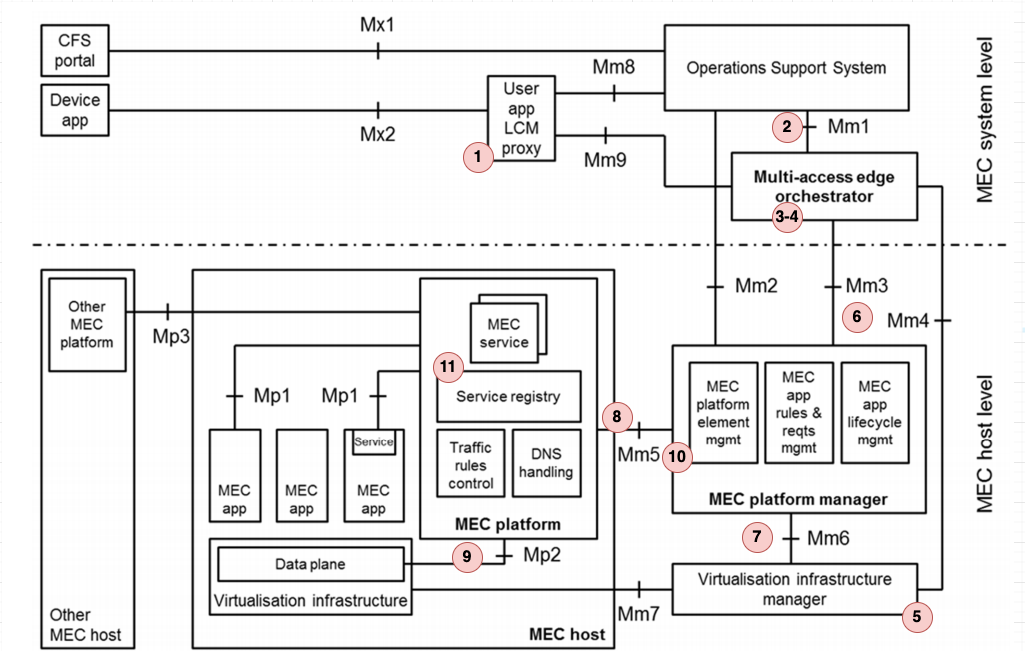
\includegraphics[width=\linewidth]{images/mec-referenzepoints.png}
  \caption{Schritte für das Starten einer MEC Anwendungen \cite{etsiMultiaccessEdgeComputinga}}
  \label{fig:ablaufmec}
\end{figure}
Dieses Unterkapitel beschreibt, wie die zuvor erläuterten Komponenten des MEC-Systems zusammenarbeiten. Die Grafik \ref{fig:ablaufmec} zeigt die 
Referenz Architektur. Wird eine neue MEC-Anwendung gestartet werden folgende Schritte durchgeführt:
\begin{enumerate}
  \item Die \acrshort{ue} Anwendung stellt eine Anfrage für das Starten einer neuen Anwendung auf dem MEC-System. Die Anfrage läuft über den 
  User App LCM Proxy. Dieser leitet diese an das \acrlong{oss} weiter.
  \item Das \acrshort{oss} gibt die Anfrage an den MEC- Orchestartor weiter.
  \item Die Anfrage für das Starten einer neuen MEC- Anwendung enthält Informationen über 
  die Anwendung und andere Informationen. Dies beinhaltet der Ort an dem die Anwendung ausgeführt werden soll, 
  andere Anwendungsregeln und Anforderungen sowie den Speicherort des Anwendungsimage, 
  falls dieses noch nicht im MEC-System vorhanden ist. 
  \item Anhand folgender Informationen wählt der MEC-Orchestartor ein geigneten MEC-Host aus:
  \begin{itemize}
    \item Latenzanforderungen an die Anwendung
    \item Anforderung an den Ort (möglichst in der Nähe des \acrshort{ue})
    \item Benötigte Speicher- und Rechenressourcen
    \item MEC-Services die für die Anwendung benötigt werden
    \item Mobilitätsanforderungen (muss die Anwendung umziehen, muss der Zustand der Anwendung umziehen)
    \item Art des Hostens der Anwendung (Handelt es sich um eine Instanz pro Benutzer eine Instanz pro MEC-Host)
    \item Informationen über den Netzbetreiber des MEC-Hosts (Kosten, Funknetztopologie)
  \end{itemize}
  Der MEC-Orchestrator wählt anhand dieser Informationen ein oder mehrere MEC-Hosts aus und startet das Initialisieren der Anwendungen.
  \item Für das Abfragen der verfügbaren Ressourcen kommuniziert der MEC-Orchestartor mit dem Virtualization Infrastruktur Manager.
  \item Wurde ein passender MEC-Host gefunden, startet der MEC Platform Manager die Anwendung. der MEC-Platform Manager erhält von dem 
  MEC-Orchestartor die Anfroderderungen der Anwendung.
  \item Der MEC-Platform Manager kommuniziert mit dem Virtualization Infrastruktur Manager um die benötigten virtualisierten Ressourcen 
  bereitzustellen. der Infrastruktur Manager läd das benötigte Image für die Anwendung runter wenn dieses noch nicht Verfügbar ist.
  \item Anschließend kommuniziert der MEC- Platform Manager mit der MEC- Platform um die Anwendung zu konfigurieren.
  \item Die MEC- Platform konfiguriert das Routing des Datenverkehrs  auf der Data-Plane der virtuellen Infrastruktur.
  \item Der MEC- Platform Manager startet die Anwendung auf der virtuellen Infrastruktur.
  \item Die Anwendung registriert sich bei der MEC-Platform in der Service Registry. Die MEC-Platform konfiguriert die DNS Regeln der 
  Anwendung und verwaltet den Zugriff auf den Persistenten Speicher.
\end{enumerate}

\newpage

\section{Integration von MEC und 5G}
In der 5G-Systemspezifikation stehen zwei Optionen für die Architektur zur Verfügung. 
Eine mit dem traditionellen Interface Ansatz und eine weitere 
bei der die Netzwerkfunktionen des Kernnetzes mithilfe einer \acrfull{sba} verbunden sind. 
Hier wird die Service Based Architecture betrachtet. Bei \acrshort{sba} können die Netzwerkfunktionen Dienste bereitstellen oder konsumieren, eine
Funktion kann auch mehrere Dienste anbieten. 
Für die effiziente Nutzung der Dienste, 
ist eine Registrierung, Service Discovery, Abmeldung sowie Authentifizierung und Autorisierung erforderlich.
Die Abbildung \ref{fig:sba} zeigt auf der linken Seite ein 5G-System in Form von \acrshort{sba}, 
die rechte Seite zeigt die MEC-Systemarchitektur aus Kapitel \ref{subsec:MEC Framework - Referenz Architektur}.
\begin{figure}
  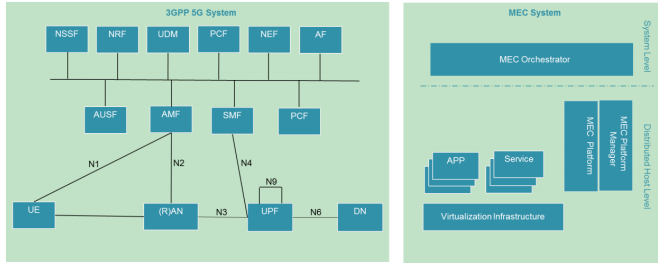
\includegraphics[width=\linewidth]{images/5GMEC-System-Architecture.png}
  \caption{5G Servicebasierte Architektur und MEC Systemarchitektur \cite{arnold5GRadioAccess2017} \cite{etsiETSIGSMEC}, \cite{etsiMultiaccessEdgeComputinga}}
  \label{fig:sba}
\end{figure}
\\
Dieser Abschnitt beschreibt, wie \acrfull{mec} in die 5G-Netzwerkumgebung integriert werden kann 
und welche Komponenten miteinander interagieren.
\\
\\
Die Netzwerkfunktionen und die Dienste die diese zu verfügungstellen, werden im 5G System in der \acrfull{nrf} registriert.
Die \acrshort{nrf} bietet damit eine Liste mit allen Diensten an. 
In einem MEC System werden die Dienste die von den MEC- Anwendungen bereitgestellt werden in der Service Registry in der MEC Platform registriert.
Will eine Netzwerkfunktion im 5G Netzwerk ein Dienst nutzen, kann diese direkt mit der Funktion die den Dienst zur Verfügungstellt interagieren,
wenn diese au­then­ti­fi­zie­rt ist. Die \acrfull{nef} im 5G System stellt auch Dienste an nicht au­then­ti­fi­zie­rte Komponenten 
zur Verfügung. Die \acrshort{nef} ist damit sehr wichtig für die Bereitstellung von Services, da sie Anfragen von nicht authentifizierten Komponenten
entgegennimmt.
\\
\\
\subsection{\acrfull{upf}}
Für die Integration von MEC in ein 5G Netzwerk, spielt die \acrfull{upf} eine wichtige Rolle. Die \acrshort{upf} ist Teil der User Plane
und ist eine Darstellung dieser in Netzwerkfunktion. Die UPF ist das Gateway zur Kontrollen und Weiterleitung von Nutzdaten. 
Sie dient als Verbindungspunkt für die mobile Infrastruktur und das Data Network (DN). Beispielsweise ist es für das packen und entpacken von 
getunnelten Daten verantwortlich. Darüber hinaus dient die \acrshort{upf} auch als Anker für die Mobilität, was besonders für das Mobilitätsmanagement wichtig ist.
\cite{Leitfaden5GCampusnetze2020}
\subsection{MEC- Kommunikation mit dem 5G Netzwerk}
Dieser Abschnitt beschreibt die Kommunikation des MEC
Plattform mit 5G-Kerndiensten.

In einem 5G System, verhält sich das MEC-System wie eine \acrfull{af} für 5G. Ist ide \acrshort{af} ein Teil des Netzbetreibers, ist diese 
Registriert als ein Teil des Kernnetzwerkes. Die AF sendet Informationen wie MEC-Application Details und Routing-Informationen 
an die \acrshort{pcf}. Diese benachrichtigt den \acrshort{smf}. Die \acrlong{smf} verwendet die Inofmrationen um neue Routing Regeln in der
aktuellen \acrshort{upf} zu hinterlegen. Ist die \acrshort{upf} nicht an der aktuellen Lage verfügbar, erstellt die \acrshort{smf} eine 
neue \acrshort{upf} und hinterlegt die routing-Regeln so, dass der Netzwerkverkehr des Endgeräts zu der MEC-Anwendung weitergeleitet wird.
\\
\\
Ist das MEC nicht Teil des Netzbetreibers, dann interagiert die \acrshort{af} mit der \acrshort{nef} um den Datenverkehr zu steuern.
Nach der Autorisierung die \acrshort{af}, sendet der \acrshort{nef} Details über das Routing an den \acrshort{smf}. Ist die \acrshort{upf}
verfügbar, fügt der \acrshort{smf} neue Routing-Regeln, ist dies nicht der Fall, wird eine neue \acrshort{upf} erstellt und die Routing-Regeln
hinterlegt.

\subsection{MEC Deployment in 5G}
\begin{figure}
  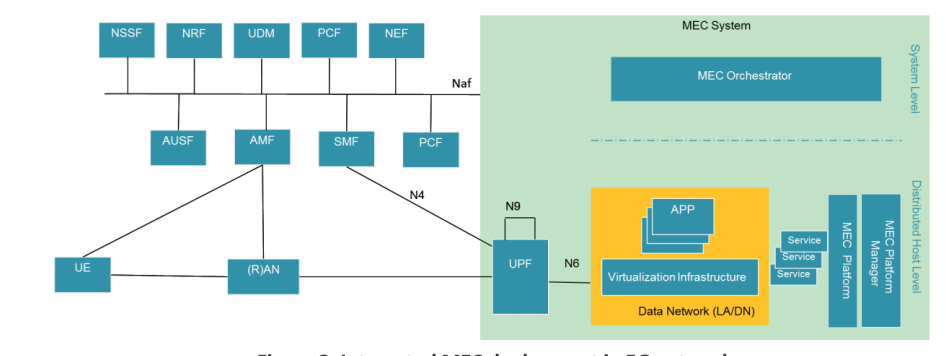
\includegraphics[width=\linewidth]{images/5GMEC-System-Architecture2.png}
  \caption{MEC in 5G \cite{etsiMultiaccessEdgeComputinga}}
  \label{fig:sba2}
\end{figure}
In dem MEC- System auf der rechten Seite, agiert der MEC- Orchestartor auf der MEC-System Ebene. Dieser interagiert über die \acrshort{nef} oder
direkt mit den einzelnen Netzwerkfunktionen des 5G Netzwerks. Auf der MEC-Host Ebene, interagiert die MEC-Platform mit den Neutzwerkfunktionen des 5G Netzwerkes.
Die MEC-Host Ebene ist meistens auf der \acrshort{up} des 5G Netzwerks, während der \acrshort{nef} als Teil des \acrshort{cp} als Systemlevel 
Funktion zentral eingesetzt wird.
Wie Abbildung \ref{fig:sba2} zeigt, befindet sich das MEC-System auf der \acrshort{cp} des 5G Netzwerkes. 
\\
\\
Das 5G-Kernnetz kann aus einem oder mehreren
UPFs, die zum Steuern des Datenverkehrs zwischen MEC und dem 5G-Kernnetz konfiguriert sind.
Alternativ kann die MEC-Plattform einen lokalem UPF bereitstellen.
In einer einzelnen \acrfull{upf}-Konfiguration können 5G-Netz und MEC-Plattform nur mit einer \acrfull{upf} verbunden werden, 
der Regeln zum Weiterleiten von Datenverkehr an MEC oder Internet / Cloud enthält. In diesem fall ist die einzelne \acrshort{upf}s Teil des 
MEC-Host.
\begin{figure}
  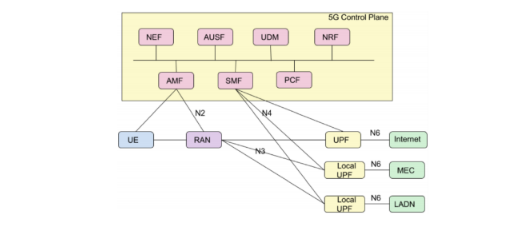
\includegraphics[width=\linewidth]{images/5g-scenarios.png}
  \caption{\acrshort{upf} in der \acrshort{up} und als Teil des MEC-Systems}
  \label{fig:sba2}
\end{figure}
In einer Konfiguration mit mehreren \acrfull{upf}s leitet eine \acrfull{upf} den Datenverkehr an die MEC-Anwendungen und 
eine anderer an Cloud- / Remote-Anwendungen weiter.
Das MEC- System kann an verschiedenen Standorten in der nähe der Base Station des 5G Netzwerkes eingesetzt werden. 

\newpage

\section{Mobilitätsmanagement in Mobile Edge Clouds}
\label{sec:Mobilitätsmanagement}
Die Mobilität von Endgeräte im \acrshort{3gpp} Netzwerken, kann dazu führen, dass ein \acrshort{ue} sich von einer 
Radio Station zu nächsten bewegt. Das Verwalten und Aufrechterhalten dieser Verbindungen in Funknetzen wird
als Mobilitätsmanagement bezeichnet und ist eine Kernkomponenten von Funknezten. 
Wird eine aktive Funkverbindung von einer Netzwerkzelle zu einer anderen weitergegeben, wird der Vorgang
der Übergabe als Handoff oder Handover bezeichnet.\\
Die Mobilität des Endgerätes kann dazu führen, 
dass sich das \acrshort{ue} zu einer anderen Zelle bewegt, 
die einem anderen MEC-Host zugeordnet ist. Es muss sichergestellt werden, dass der Datenverkehr
richtig geroutet wird um das Ziel zu erreichen.
Entfernt sich das Endgerät weiter vom Ort der MEC-Anwendung, 
kann dies dazu führen, dass die Latenz sich erhöht und die Deshalb ist es wichtig, dass je nach Anwendung,
die laufende Anwendungsinstanz verschoben wird um die Latenz Anforderungen weiterhin zu erfüllen. \\
Die Häufigkeit eines wechsel der MEC Hosts, hängt stark von dem 
Einsatz ab. Bei der Verwendung von MEC für Autonomes Fahren treten häufiger Handover Event ein, wie bei
beispielsweise in dem Szenario einer Smart Factory.\\
Die Mobilität eines \acrshort{ue}s kann in weitreichenden MEC-Systemen vorhergesagt werden und die einzelnen MEC-Host demnach konfiguriert werden,
dennoch muss der Zustand der Anwendung übertragen werden.
Dieses Kapitel beschreibt wie verschiedene Handoff Events ablaufen. \cite{etsiMultiaccessEdgeComputinga}

\subsection{Verschieben der Anwendung und dessen Zustand}
Bewegt sich das \acrshort{ue} im Funknetz und ist möglicherweise ein anderer Ziel MEC-Host geeigneter als der aktuelle
MEC-Host, muss die Anwendung umziehen. Die MEC-Anwendungen werden in zustandslose und zustandsbehaftete Anwendungen eingeteilt.
Handelt es sich um eine zustandsbehaftete Anwendung, 
erfordert das Umziehen der Anwendung, ein synchronisieren des Zustands zwischen der aktuellen und der
verschobenen Anwendungsinstanz, um Kontinuität zu gewährleisten zu können.
\\
\\
Das Synchronisieren des Zustands muss bei dem Entwickeln der Anwendungen berücksichtigt werden. Diese muss so konzeptiert werden, 
dass die Anwendung in mehreren Instanzen auf unterschiedlichen MEC-Hosts betrieben werden kann. 
Für das Synchronisieren muss die Anwendungen das Einfrieren des Zustands und kopieren von einer Quell- Anwendung 
zu einer Zielanwendung unterstüzen. 
Läuft die Anwendung noch nicht auf dem Ziel Host, muss diese initalisiert und gestartet werden.
Nachdem die Anwendung gestartet ist, startet der Umzugsvorgang und der Zustand wird von dem aktuellen 
Host zu dem Ziel MEC-Host übertragen. Wenn der Zustand vollständig übertragen ist, stoppt die aktuelle Instanz
und die Ziel Instanz übernimmt das kommunizieren mit dem Endgerät. \cite{DevelopingSoftwareMultiAccess}
\\
Für das Erkennen von \acrshort{ue} Mobilität zu einer neuen Zelle, abonniert die MEC Platform Radio Network Informationen die von dem \acrfull{rnis} zu
Verfügung gestellt werden. Mithilfe dieser Informationen können \acrshort{ue}s identifizieren werden, bei denen eine Zelländerung auftritt 
und bestimmen es kann bestimmt werden, ob diese sich aus dem Versorgungsbereich des aktuellen MEC-Hosts herausbewegen.
\subsection{Aktualisierung des Routings für Mobilitätsupport}
\subsubsection{Problem}
Das MEC-System ist in der Lage flexibel \acrlong{up} Funktionen anzupassen je nach den Anforderungen oder Regeln des MEC-Systems 
und dem Zustand des Netzwerkes. Für das Mobilitätsmanagement ermöglicht dies, das flexible lenken des Datenverkehrs auf der \acrshort{up}
um die Verbindung zwischen dem Endgerät und der Anwendungsinstanz auf dem MEC-Host aufrecht zu halten. Soll die Anwendungsinstanz
beispielsweise zu einem neuen MEC-Host migriert werden und dieser ist nicht in der Lage die Instanz zu hosten, kann der aktuelle
MEC-Host noch einen zufriedenstellenden Service anbieten.
\begin{figure}
  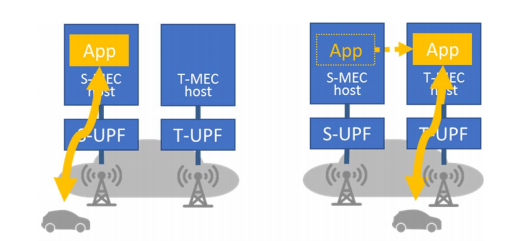
\includegraphics[width=\linewidth]{images/Verschieben_Instanz.png}
  \caption{Handover vom MEC-Host zum Ziel-MEC-Host}
  \label{fig:Verschieben_Instanz}
\end{figure}
\\
Bewegt sich das Endgerät kann es zu einem gNB Handover kommen, was zu einer Änderung in der \acrshort{upf}s Ebene führt. 
Bei Bedarf wird der Zustand zu der Instanz in dem Ziel-MEC-Host übertragen und das Routing wird für das Endgerät angepasst, 
was in der Grafik \ref{fig:Verschieben_Instanz} zu sehen ist.
Kann der Ziel MEC- Host die Anwendung nicht hosten, weil dieser nicht über ausreichend Ressourcen verfügt oder nicht den gewünschten Service
erfüllt, kann der Zustand einer laufenden Anwendungsinstanz nicht von dem S-MEC-Host zum Ziel-MEC-Host übertragen werden. 
Wenn dies der Fall, muss das Routing
trotzdem aktualisiert werden. Die Anwendungsdaten werden entweder über den Ziel-MEC-Host (Bild 2 in Abbildung \ref{fig:mecerror}) 
oder über die \acrshort{upf}s des Ziel und ursprünglichen MEC-Hosts geleitet (Bild 3 in Abbildung \ref{fig:mecerror}).
\begin{figure}
  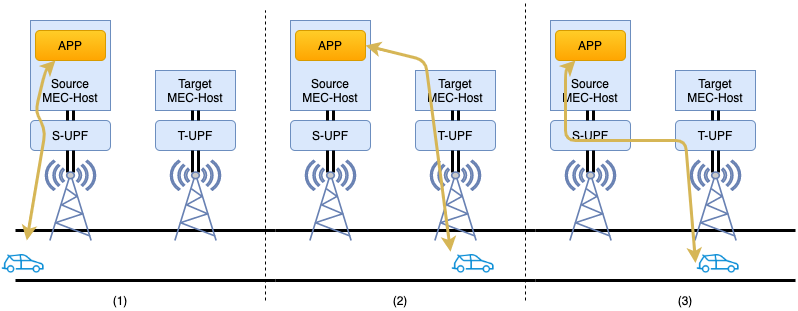
\includegraphics[width=\linewidth]{images/MEC_host_Error.png}
  \caption{Routing wenn der Ziel-MEC Host die Anwendung nicht hosten kann}
  \label{fig:mecerror}
\end{figure}
Unabhängig davon, ob die Anwendungsinstanz erfolgreich auf den Ziel-MEC-Host übertragen wurde oder nicht, 
der Verkehrspfad wird entsprechend aktualisiert. \cite{etsiMultiaccessEdgeComputinga}
\subsubsection{Aktualisieren des Routings}:
Für das Aktualisieren und Aufrechterhalten der Routen, ist die \acrlong{af} verantwortlich.
Die \acrfull{af} interagiert mit \acrshort{cp},  um das Routing zu beeinflussen. 

\begin{figure}
  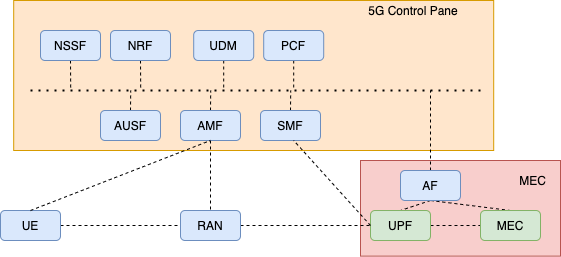
\includegraphics[width=\linewidth]{images/AF_5G.png}
  \caption{Application Function in 5G}
  \label{fig:AF_GG}
\end{figure}

Die \acrfull{af} erfasst Informationen über das 5G Netzwerk und unterstützt so die Mobilität von Anwendungsinstanzen. 
Dies ermöglicht in einem 5G-System eine flexiblere Bereitstellung der Data-Plane, um Edge-Computing nativ zu unterstützen.
Die Abbildung \ref{fig:AF_GG} zeigt die \acrshort{af} in einer \acrlong{sba}.
\\
\\
\acrshort{etsi} definiert für das Anpassen des Routings mithilfe der \acrshort{af} den sogenannten \textit{Application Function influence on traffic routing} Prozess.
Startet ein MEC-System diesen Prozess benötigt es folgende Parameter:
\begin{itemize}
  \item \acrshort{ue} Identifikator, eindeutig für das Endgerät
  \item Mögliche Orte für die Anwendung, Data Network Access Identifier (DNAI) wird benötigt um die Ziel UPFS zu erlangen.
  \item AF-Transaktionskennung, wird von der \acrshort{af} generiert
  \item Beschreigung des Datenverkehrs, dazu gehören IP-Adressen, Zieladressen und Data Network Name (DNN)
\end{itemize}
\begin{figure}
  \centering
  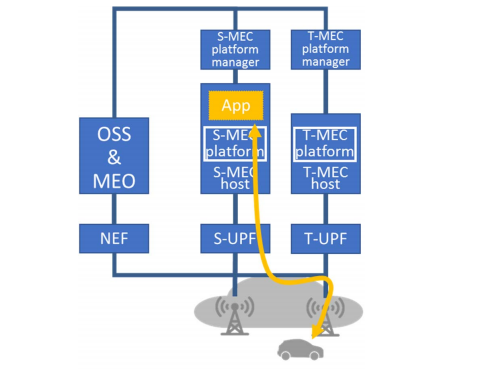
\includegraphics[width=7cm]{images/Datenverkehr_Update.png}
  \caption{Komponenten für die Aktualisierung des Routings}
  \label{fig:Datenverkehr_Update}
\end{figure}
Mithilfe dieser Parameter kann der Prozess des umleiten gestartet werden.
Abbildung \ref{fig:Datenverkehr_Update} zeigt wie die einzelnen Komponenten zusammenarbeiten um ein benötigte Aktualisierung des Datenverkehrs durchzuführen.
Die Kommunikation mit dem MEC-System läuft dabei über die \acrshort{nef}. Diese kommuniziert mit dem MEC-Orchestartor welcher
die Informationen auf MEC-Host Ebene an den Platform Manager weitergibt. \cite{etsiMultiaccessEdgeComputinga}  \cite{balasubramanianMobilityManagementArchitecture2019}
\begin{figure}
  \centering
  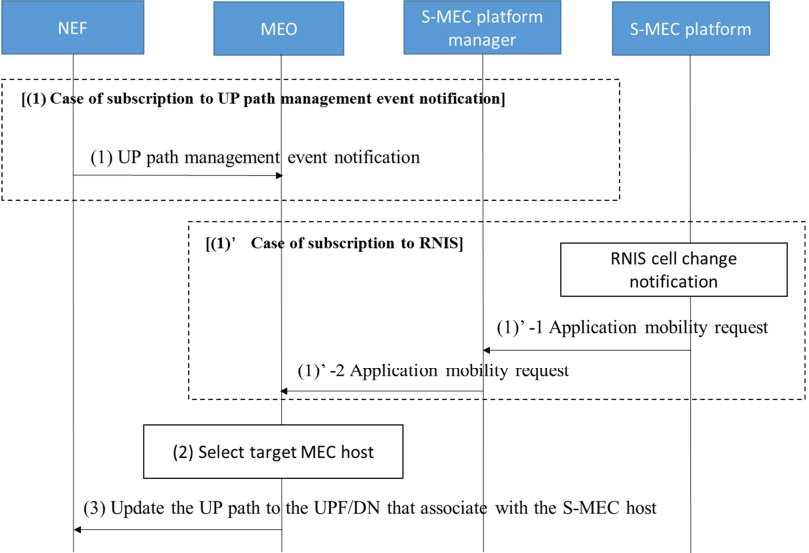
\includegraphics[width=9cm]{images/Datenverkehr_Ablauf.png}
  \caption{Ablauf der Aktualisierung}
  \label{fig:Datenverkehr_Ablauf}
\end{figure}
Für das Aktualisieren des Routings werden folgende Schritte (Abbildung \ref{fig:Datenverkehr_Ablauf}) durchgeführt:
\begin{enumerate}
  \item Der \acrfull{meo} abonniert über \acrshort{nef}, \acrshort{up} Event Mittelungen. 
  Der \acrshort{meo} erhält daher eine Mitteilung das sich die \acrshort{ue} und \acrshort{dn} des
  \acrshort{ue}s aufgrund der Mobilität verändert haben.
  \item Die Quell-MEC-Plattform (S-MEC-Plattform) abonniert dem \acrshort{ue} zugeordnete Zellenänderungsbenachrichtigung. 
  Nachdem die S-MEC-Plattform eine Nachricht erhalten hat, bestimmt diese, ob das \acrshort{ue} die Zelle verlassen hat. 
  Ist dies der Fall sendet die S-MEC-Plattform eine Mobilitätsanfrage an den \acrshort{meo}.
  \item Der \acrshort{meo} wählt ein Ziel-MEC-Host für die Anwendung aus.
  \item In dem Fall, in dem der Ziel-MEC-Host aus nicht verfügbar ist, beispielsweise nicht ausreichend Ressourcen hat,
  wird die Anwendungsinstanz auf dem S-MEC-Host fortgesetzt und der vorhandene Pfad wird mittels der \acrshort{upf} zum S-MEC-Host umgeleitet.
  \item Der \acrshort{meo} sendet eine Aktualisierung an den S-MEC-Plattformmanager und dem T-MEC-Plattformmanager
\end{enumerate}
Diese Schritte ermöglichen eine kontinuirliche Verbindung zwischen \acrshort{ue} und MEC-Anwendung, unabhängig ob diese sich beim S-MEC-Host oder Z-MEC-Host befindet.
\newpage
\subsection{Ping-Pong Handover}
\subsubsection{Problem}
Ping-Pong-Übergaben treten auf, wenn ein Endgerät von einer Zelle zur nächsten wechselt, dann aber wieder in die ursprüngliche 
Zelle zurückgeht. Befindet sich ein Endgerät zwischen zwei Zellen, hat dies die Folgen, das es zwischen den zwei Hosts
hin und herspringt. Daher die Bezeichnung Ping-Pong Handover.
\begin{figure}
  \centering
  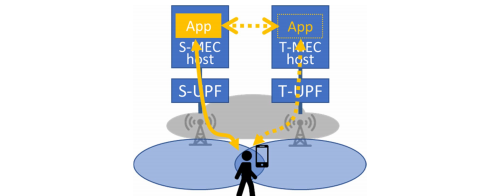
\includegraphics[width=6cm]{images/pingpong.png}
  \caption{Ping Pong Handover}
  \label{fig:pingpong}
\end{figure}
\subsubsection{Lösung}
Für das Lösen des Ping-Pong Problems im MEC- System, schlägt \acrshort{etsi} eine Verringerung der Migrationsevent die vom MEO durchgeführt werden vor.
\begin{enumerate}
  \item Der \acrshort{meo} wird Benachrichtigt, wenn es zu einem Ping-Pong Handover kommt, das zahlreiche Migrationen von MEC-Anwendung verursacht. Das
  Ping-Pong event wird dabei durch eine Vielzahl von Events der UPFS Erkannt.
  \item Nach dem Erkennen eines Ping-Pong Events, startet der \acrshort{meo} den \textit{Ping-Pong Handover Migration} Prozess. Dieser verändert die \acrshort{upf}
  so, dass diese sich immer zur S-MEC-Anwendung verbindet, unabhängig von der Verbindungsqualität des UEs. Dies reduziert die Anzahl der Migrationen
  zwischen Source-MEC-Host und Target-MEC-Host, auch wenn das \acrshort{ue} sich oft zwischen Netzbereichen der Hosts wechselt. Das \acrshort{ue} kommuniziert weiterhin
  mit der Anwendung im S-MEC über die Source-UPF. Abildung \ref{fig:pingpongrouting} zeigt dies.
  \item Der \acrshort{meo} wartet auf das sogenannte \textit{Ping-Pong Recovery Event}. Dieses signalisiert, dass das \acrshort{ue} sich nicht mehr zwischen zwei
  Aufgabenbereichen der MEC-Hots befindet.
  \item Nach dem \textit{Ping-Pong Recovery Event} setzt der \acrshort{meo} das Routing im UPFs wieder auf den ursprünglichen Zustand zurück.
\end{enumerate}
So kann mithilfe des \textit{Ping-Pong Handover Migration} und \textit{Ping-Pong Recovery Event} mit dem Ping-Pong Problem
in einem MEC-System umbegangen werden.
\begin{figure}
  \centering
  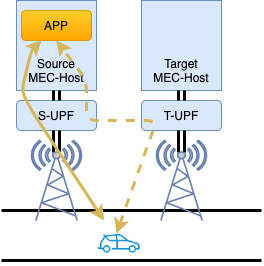
\includegraphics[width=6cm]{images/pingpongrouting.png}
  \caption{Angepasstes Routing}
  \label{fig:pingpongrouting}
\end{figure}
\newpage


\section{Multi-Access Edge Computing Scenarios}
\label{sec:Anwendungen}
Folgendes Kapitel beschreibt unterschiedliche Use-Cases und Szenarios für die Verwendung von MEC.\cite{patelContributorHuaweiVice}
\subsection{Cloud-Gaming, Remote Desktop}
\label{subsec:Cloud-Gaming}
Computer Spiele werden immer populärer, aber die meisten Online Multiplayer Spiele benötigen eine geringe 
Latenz über das Netzwerk. Dies ist meistens nicht für mobile Endgeräte möglich, da sich die Server nicht im \acrshort{ran} befindet und so
nicht in der Nähe des Endgerätes.
\\
\\
Bringt man die Spielserver in die Nähe des Funknetzes, ermöglicht dies das spielen von Spielen die eine geringe Latenz benötigen
für mobile Nutzer. 
Die Verwendung ist dabei nicht auf Spiele beschränkt und kann auch für andere Anwendungen von Vorteil sein, 
die eine geringe Latenz erfordern. Beispielsweise können durch die geringe Latenz mobile Endgeräte mit \textit{Remote Desktop} auf
Virtuelle Maschinen zugreifen und benötigen so keine lokale Rechenressourcen. Dies erlaubt Tablets mit wenig Rechenleistung als 
\textit{Thin Client} sich mit geringer Latenz mit einer \acrshort{vm} zu verbinden.
Es kann sich ein oder mehrere Nutzer mit der VM auf dem Server verbinden. 
Der Nutzer startet für das Verbinden
die Anwendung lokal auf dem Endgerät und diese Verbindet sich mit der Cloud. Nutzen mehrere Benutzer eine Anwendungs Instanz auf dem 
gleichen MEC-HOST, ist die Latenz auch unter den Nutzern geringer. Bei einem Onlinespiel ist die Verzögerung zwischen zwei Spielern
auf dem gleichen Server sehr gering. Wird eine Remote-Desktop anwendung von mehreren Nutzern in dem gleichen MEC-Host verwendet, 
ist die Latenz gering und die Bandbreite groß. 
So können zu für kolaborative Arbeiten beispielsweise große Datein mit hoher Bandbreite geteilt werden, oder kolaborative Programme wie
ein geteiltes Whiteboard mit geringer Latenz genutzt werden, auch wenn die Nutzer mobil sind. \cite{etsiMultiaccessEdgeComputing}
\\
\\
Benötigen die Anwendungen eine geringe Latenz, kann auch das Rendern der Videospiele oder Virtuellen Maschine auf dem MEC-Host 
durchgeführt werden. Die Endgeräte decodieren dann nur den Videostream der MEC-Anwendungen und senden die Steuerungseingaben in die Cloud.
Gerade bei Spielen reichen dann \textit{Thin Clients} aus und es werden keine leistungsstarke lokale Ressourcen benötigt. 
Dies ermöglicht das spielen von grafikintensiven Online-Spielen auf Smartphones. \cite{chinamobileztePoweredSA5G}
\\
\\
Wenn sich ein \acrshort{ue} mit einem Funkknoten verbindet, der nicht demselben MEC-Host zugeordnet ist, 
auf dem die Anwendung ausgeführt wird (z. B. nachdem sich das Endgerät von dem wegbewegt hat), 
muss sichergestellt sein, dass die Konnektivität zwischen dem \acrshort{ue} und der Anwendung aufrechterhalten wird. 
Um die Latenzanforderungen und damit eine gute Benutzererfahrung aufrechtzuerhalten, 
muss der \acrshort{meo} die Anwendung auf einen anderen MEC-Host, der in der Nähe des \acrshort{ue}s ist, verschieben. 
Dabei ist es wichtig, dass die Verbindung aufrechterhalten wird. Gerade bei dem mobilen spielen von Online-Spielen
ist dieser Schritt sehr wichtig, da es zu frustrierenden Benuzung kommt. \cite{etsiETSIGSMEC} 
\\
\\
Aktuell werden Cloud-Gaming-Services wie Googles \textit{Stadia} immer verbreiteter. Das Streamen von Videospielen ist
allerdings nur im Heimnetzwerk möglich. 5G und MEC könnten es ermöglichen auch von Mobilen Endgeräten Cloud-Gaming-Services zu Nutzen,
und die Latenz zu verbessern. \cite{etsiMultiaccessEdgeComputing}
\subsection{Smart Cities}
\label{subsec:Smart Cities}
In einer Smart City werden Technologien aus den Bereichen Energie, Mobilität, Stadtplanung, 
Verwaltung und Kommunikation so miteinander vernetzt, dass sich die Lebensqualität für die Bewohner verbessert. 
Gleichzeitig profitiert die Nachhaltigkeit der Stadt. Dies wird immer wichtiger, da die Bevölkerungszahlen in 
Städten immer weiter zunehmen.
Darüber hinaus wird der Bevölkerungsanstieg die städtische Infrastruktur aufgrund einer 
exponentiellen Zunahme der Daten, die von verschiedenen Geräten wie Smartphones, Sensoren und Kameras generiert werden, 
vor weitere Herausforderungen stellen. 
\\
\\
Die Vielzahl von Daten die von einer Smart-City generiert werden müssen verarbeitet und ausgewertet werden. Dies kann durch lokalen Rechenressourcen
direkt an der Datenquelle durchgeführt werden, was aber sehr teuer ist und praktikabel ist. 
Um die Notwendigkeit von dedizierter teurer Computerhardware zu beseitigen, wurde Cloud-Computing eingeführt. Cloud-Computing führt allerdings
zu einer hohen Latenz was gerade im Kontext von Smart-Cities die Vielzahl von Echtzeitdaten generieren nicht optimal ist.
Des Weiteren belastet Cloud-Computing das gesamte Netzwerk der Stadt. 
Wenn die Rechenleistung näher an der Datenquelle liegt, könnenn die Daten mithilfe von Edge-Computing und 5G schneller analysieret
und auf Anfragen geantwortet werden, ohne das gesamteNetz zu belasten.
\\
\\
Die Verwendung von Kameras in einer Smart-City ist vorallem durch die Verfügbar Bandbreite eingeschränkt. 
Hochauflösende Lifestreams von Kameras erfordern viele Ressourcen für die Analyse und viel Speicherplatz. 
Dies macht das Einsetzen von HD-Kameras unter den gegenwärtigen Bedingungen schwierig.
Das Einsetzen von \acrlong{mec} kann dies ändern. Ein MEC-Systems ermöglicht das schnelle analysieren und auswerten von
Videoinformationen und Speichern im MEC-HOST, in der Nähe der Kamera. Gleichzeitig ermöglicht  5G eine geringe Latenz und eine 
hohe Datenrate. Durch die gewonnene Mobilität, ist es beispielsweise möglich das Kameras von Polizisten und Polizistinnen über das 5G Netz
übertragen und in Echtzeit ausgewertet werden. Die Firma \textit{Dragon Law Enforcement} arbeitet aktuell an einer Spracherkennung.
Diese passt sich den Akzenten an und reduziert den Lärm, um den Beamten dabei zu helfen, 
Protokolle sehr genau und effizient zu erstellen. \cite{5GGivingLaw}
\\
\\
Ein weiter Use-Case im Bereich Smart-City ist die \textit{Vehicle-to-Infrastructure} Kommunikation.
Bei der Vehicle-to-Infrastructure werden Daten vom Fahrzeug und Sensoren an eine Infrastruktur gesendet, um die Sicherheit zu erhöhen und 
Risikosituatonen frühzeitig zu erkennen. 
Die Kommunikation zwischen Fahrzeug und der Infrastruktur erfordert eine geringe Latenz, 
die je nach Anwenungsfall unter 10 ms liegen muss. 
Gefahrenmeldungen wie Unfälle, stehengebliebene Fahrzeuge oder ein Stau können in in Echtzeit über 5G übertragen werden.
MEC kann hier eingesetzt werden, um die Fahrzeuge mit einer verteilten Cloud zu verbinden. So können MEC Anwendungen auf den MEC-Host 
gehostet werden, die Daten aus Fahrzeugen und Sensoren analysiert. Wird eine Gefahr erkannt, kann der MEC-Host dies mit einer
geringen Latenz an andere Fahrzeuge Broadcasten. 
Dies ermöglicht einem smarten Auto innerhalb von Millisekunden Daten zu empfangen, 
sodass der Fahrer auf eine Gefahr reagieren und ausweichen kann.
\\
\\
Besonders für die \textit{Vehicle-to-Infrastructure} Kommunikation eignet sich ein MEC-System. Da Fahrzeuge mobil sind, wechseln sie
oft den Netzwerkknoten. Das MEC-System ist für so eine Mobilitätsaufgabe ausgelegt. Gerade bei diesem Use-Case betreibt 
jeder MEC-Host die gleiche Anwendung. Beispielsweise eine Anwendung zur Analyse der Fahrzeugdaten. Das macht das wechseln von MEC-Hosts sehr effizient,
da kein Image geladen werden muss und die Anwendung auf dem Ziel-MEC schon läuft. Bei einer Gefahrensituation ist es wichtig, dass die
umliegenden Fahrzeuge schnell Benachrichtigt werden. Da aufgrund der geographischen Lage die Fahrzeuge mit dem gleichen MEC-Host
kommunizieren, wie das Fahrzeug das eine Gefahr erkannt hat, ist das Benachrichtigen mit einer geringer Latenz möglich. 
\\
\\
Auch für die \textit{Vehicle-to-Vehicle} Kommunikation eignet sich MEC. Die Daten eines Fahzeuges können mit geringer Latenz
an einen MEC-Host gesendet werden, analysiert und an andere Fahrzeuge im gleichen MEC-host weitergeleitet werden.
\subsection{Smart-Factory}
Die Smart-Factory steht im Mittelpunkt der Industrie 4.0 und bezeichnet eine Produktionsumgebung, die sich selbst organisiert. 
Zur Produktionsumgebung gehören die Fertigungsanlagen und die Logistiksysteme. Die Produktionsumgebung ist automatisiert und erfordert
nicht das Eingreifen eines Menschens. 
Im Mittelpunkt einer Smartfactory steht die intelligente Vernetzung von Maschinen und das hergestellte Produkt. 
Das Produkt teilt die für die Fertigung benötigten Informationen der Smart Factory mit. 
Anhand dieser Informationen stellen sich die Maschinen automatisch ein, um das gewünschte Produkt zu fertigen. 
In vielen Fällen findet dafür eine drahtlose Kommunikation zwischen Produkten und Anlagen statt.  \cite{gundall5GEnablerIndustrie2018}
\\
\\
Für die Smart-Factoy bietet sich ein MEC-System an. 5G besitzt die Möglichkeit eines Privaten Netzes. 
So kann ein Netzwerk \textit{On-permise} bie einem Unternehmen zu Verfügung gestellt werden. 
Maschinen und Produkte können Daten via 5G an MEC-Hosts senden.
Ein Smart Factory besteht aus einer Vielzahl von \acrfull{iot} Geräten. Dide Menge an Daten die dadruch 
generiert wird, kann nicht über das \acrshort{wan} zu einer zentralen Cloud gesendet werden. Ein MEC-System ist reduziert die Latenz
und die Auswirkungen auf das Netzwerk. Des Weiteren wird die Sicherheit erhöht, da die Daten lokal bleiben und nicht über 
das \acrshort{wan} versendet werden. Auf dem MEC-Host können die Daten der \acrshort{iot} Geräte in Echtzeit analysiert werden. Beispielsweise können
Maschine Learning Modelle für die Optimierung der Produktion eingesetzt werden. Der MEC-Host, kann die ankommenden Daten auch filtern und Entscheidungen über
die Relevanz der ankommenden Daten treffen. Nur die relevanten Daten können dann zu einer zentralen Cloud weitergeleitet werden. Die Vorauswahl der Daten entlastet
das Netz und verursacht weniger kosten.
\\
\\
Eine mögliche Anwendung für MEC in einer Smart-Factory ist das Einsetzen von Kameras zur Qualitätssicherung.
Für das Erkennen von fehlern in Produktionsteilen, müssen hochauflösende Kameras verwendet werden. Der hohe Datenstrom
kann über 5G an den MEC-Host gesendet werden. Dieser analyisiert das Bildmaterial auf fehler. Wird ein fehler erkannt,
kann der MEC-Host andere Maschine benachrichtigen, die das beschädigte Teil entfernt. Je nach der Geschwindigkeit der Produktion,
es wichtig das dies mit einer geringen Latenz passiert. \cite{etsiMultiaccessEdgeComputing}
\\
\\
Huawai arbeitet zusammen mit China Mobile an einer \textit{5G Connected Factory}. Hier soll die Anlage mithilfe 
einer Edge Cloud die Produktion verbessern und über Kameras Fehler erkennen. \cite{WhatNextgenFactory}

\newpage

\section{Fazit und Ausblick}
Diese Seminararbeit gibt ein Überblick über die MEC-Technologien. Es wurden erläutert wie die 
zugrunde liegenden
Technologien wie \acrshort{sdn}, \acrshort{nfv}, \acrshort{nfvi}, Network-Slicing und \acrshort{cups}
dem 5G Netzwerk helfen, die Latenz von MEC-Anwendungen zu verringern, was gleichzeitig die Nutzung der
Netzwerkressourcen optimiert und so die Benutzererfahrung verbessert. In dieser Arbeit wurde auch gezeigt, 
wie das MEC-Framework und die MEC-Referenz Architektur mit Herausforderungen wie die Mobilität des Benutzers
umgehen. Dabei wurde ausführlich auf die Integration von MEC in das 5G Netzwerk eingegangen.
\\
\\
Früher als Mobile Edge Computing bekannt, ist Multi-Access Edge Computing eine der 
wichtigsten Säulen für 5G und  definitiv eine der vielversprechendsten Technologien, 
um Cloud-basierte Anwendungen und Dienste in das Geschäft von Netzbetreibern zu integrieren.
MEC ist eine der wichtigsten Technologien für 5G-Systeme, 
da es zu einer geringen Latenz und zur Kapazitätsverbesserung und Kernnetzwerk führt. 
\\
\\
\acrlong{etsi} hat eine Vielzahl von MEC-Standards veröffentlicht,die eine Cloud-Umgebung am Rand des 
Netzwerkes ermöglicht. Der Erfolg von 5G hängt im wesentlichen von der Ausrichtung der Technologien ab.
\acrshort{etsi} definiert ausführlich die Managemen- und Orchestrierungssysteme für den Lifecyclemanagement der 
Anwendungen sowie deren Mobilität. Darüber hinaus sind die API Schnittstelle der Services und die Integration
von MEC in 5G ausführlich definiert. 

\subsection{Ausblick}
Neben dem Ausbau des 5G Netzes, ist bei der Einführung von \textit{MEC} Systemen, 
die Standardisierung sehr wichtig.  \cite{abdullahSegmentRoutingSoftware21}
\subsection{Angebote}
\label{subsec:Angebote}
\label{sec:Ausblick}

% -------------------------------------------------------------------------------------------------

% -------------------------------------------------------------------------------------------------
\newpage
% Normaler LNCS Zitierstil
%\bibliographystyle{splncs}
\printbibliography[heading=bibintoc]

\end{document}
